%!TEX root = main.tex
\section{Results}
\label{sec:results}

\subsection{Backbone Performance}
\label{sec:results_backbones}

Table~\ref{tab:backbones_full} reports the test performance of the four
Vietnamese and five English backbones.  For Vietnamese,
\model{sensitiveai-vi-dlr2stage} achieves the highest macro-F1 (0.6638), while
\model{sensitiveai-vi-custom} (0.6575) is selected for fusion analysis because
its net change is the most balanced (23 corrections vs 15 regressions).  For
English, \model{sensitiveai-en-stage2} leads with macro-F1 0.7722 and accuracy
0.9080.  English backbones substantially outperform Vietnamese ones on macro-F1
(averaging ~0.76 vs ~0.66) primarily due to higher OFFENSIVE F1 (0.94 vs 0.44),
reflecting the larger clean/offensive balance in Davidson vs ViHSD.

\subsection{Rule Engine Standalone Performance}
\label{sec:results_rule}

Standalone rule engines operate with thresholds tuned on validation.
\begin{itemize}
    \item \textbf{Vietnamese rule engine} (668 entries, thresholded): accuracy
          0.5999, macro-F1 0.3452, HATE F1 0.2911, OFFENSIVE F1 0.0000 (missing
          rules for milder offenses), CLEAN F1 0.7444.
    \item \textbf{English rule engine} (123 seed entries in evaluation,
          upgraded to 818 in combined): accuracy 0.7058, macro-F1 0.5036,
          HATE F1 0.1782, OFFENSIVE F1 0.8063, CLEAN F1 0.5264.
\end{itemize}
Standalone rules alone are insufficient for robust moderation (failing on
OFFENSIVE in VI and HATE in EN), validating the hybrid design.

\subsection{Fusion Variants on Vietnamese}
\label{sec:results_fusion}

Table~\ref{tab:fusion_variants} (from the focused ViHSD study) shows that global
$\alpha$ fusion improves macro-F1 slightly (0.6583), per-channel $\alpha$ reaches
0.6593, and per-channel $\alpha$ + thresholds reaches 0.6602 (+0.0027 over AI).
The paired-bootstrap difference is $-0.0027$ ($[-0.0079, +0.0027]$, $p=0.29$) and
McNemar $p=0.26$, confirming accuracy neutrality.

\begin{table}[ht]
\centering
\scriptsize
\setlength{\tabcolsep}{3pt}
\caption{Decision-level variants for the focused Vietnamese backbone
(\model{sensitiveai-vi-custom}) on the ViHSD test split (6{,}680 comments).
Every variant reads the same frozen scores; only the mixing and decision rule
differ. The last row is the paper's primary system. \emph{Per-class columns are
F1}; the best macro-F1 is in bold. The two rule-only rows are scored inside
the fusion pipeline on the renormalised rule scores; the standalone rule
engine, with its own thresholds, is reported in the text.}
\label{tab:fusion_variants}
\begin{tabular}{lccccc}
\toprule
System & Acc. & Macro-F1 & \hate & \off & \clean \\
\midrule
AI only (argmax)                      & 0.8762 & 0.6575 & 0.5830 & 0.4493 & 0.9403 \\
Rule only (argmax)                    & 0.8494 & 0.4714 & 0.4867 & 0.0000 & 0.9274 \\
Rule only (frozen thresholds)         & 0.8421 & 0.5258 & 0.4102 & 0.2389 & 0.9284 \\
\midrule
Fusion, global $\alpha$ (argmax)      & 0.8769 & 0.6583 & 0.5851 & 0.4490 & 0.9408 \\
Fusion, global $\alpha$ (thresholds)  & 0.8769 & 0.6583 & 0.5851 & 0.4490 & 0.9408 \\
Fusion, logistic meta-classifier      & 0.8626 & 0.6513 & 0.5818 & 0.4379 & 0.9341 \\
Fusion, per-channel $\alpha$ (argmax) & 0.8774 & 0.6593 & 0.5882 & 0.4488 & 0.9408 \\
Fusion, per-channel (thresholds)      & 0.8774 & \textbf{0.6602} & 0.5906 & 0.4494 & 0.9407 \\
\bottomrule
\end{tabular}
\end{table}

\subsection{End-to-End Bilingual Evaluation (1000 Mixed Samples)}
\label{sec:e2e}

Evaluating the full pipeline (LanguageDetector $\to$ LanguageAwareTokenizer $\to$
RuleEngine $\to$ mDeBERTa $\to$ LangAwareFusion at $\alpha=0.70$) on 500 VI and
500 EN samples yields the aggregate and per-language metrics in
Tables~\ref{tab:e2e_aggregate} and \ref{tab:e2e_per_lang}.

\begin{table}[H]
\centering
\caption{End-to-end bilingual pipeline performance (1000 mixed samples)}
\label{tab:e2e_aggregate}
\begin{tabular}{lcc}
\toprule
Metric & Value & 95\% CI (bootstrap) \\
\midrule
Accuracy          & 0.8700 & [0.849, 0.891] \\
Macro F1          & 0.7829 & [0.7465, 0.8176] \\
Weighted F1       & 0.8701 & [0.849, 0.891] \\
HATE F1           & 0.5529 & [0.458, 0.639] \\
OFFENSIVE F1      & 0.8824 & [0.857, 0.905] \\
CLEAN F1          & 0.9134 & [0.895, 0.931] \\
Macro ROC-AUC     & 0.9200 & --- \\
\bottomrule
\end{tabular}
\end{table}

\begin{table}[H]
\centering
\caption{Per-language breakdown on the 1000 mixed samples}
\label{tab:e2e_per_lang}
\begin{tabularx}{\textwidth}{l@{\extracolsep{\fill}}cccccr}
\toprule
Language & Acc. & Macro F1 & \hate{} F1 & \off{} F1 & \clean{} F1 & $n$ \\
\midrule
Vietnamese & 0.8600 & 0.6500 & 0.6095 & 0.4118 & 0.9287 & 500 \\
English    & 0.8800 & 0.7430 & 0.4615 & 0.9247 & 0.8427 & 500 \\
\bottomrule
\end{tabularx}
\end{table}

Vietnamese has stronger HATE detection (0.61 vs 0.46) due to the dense 668-entry
lexicon, while English dominates OFFENSIVE (0.92 vs 0.41) due to Davidson dataset
alignment.

\subsection{Latency and Throughput Profile}
\label{sec:latency}

Table~\ref{tab:latency} reports per-request latency across the 1000 mixed
samples.

\begin{table}[H]
\centering
\caption{Per-request latency breakdown (ms) over 1000 mixed samples}
\label{tab:latency}
\begin{tabularx}{\textwidth}{Xccccc}
\toprule
Pipeline Stage & Mean & Median & P95 & Max & Thr. (req/s) \\
\midrule
Routing & 6.85 & 4.41 & 6.69 & 2157 & 146k \\
AI Inference & 4.59 & 4.59 & 4.59 & 4.59 & 217k \\
Fusion & 0.14 & 0.14 & 0.19 & 1.37 & 6.9M \\
\midrule
\textbf{Total} & \textbf{11.58} & \textbf{9.14} & \textbf{11.47} & \textbf{2162} & \textbf{86k} \\
\bottomrule
\end{tabularx}
\end{table}

End-to-end throughput reaches ~86k req/s on a single laptop GPU, well within
real-time moderation SLAs.

\begin{figure}[H]
\centering
\begin{minipage}{0.95\textwidth}
    \centering
    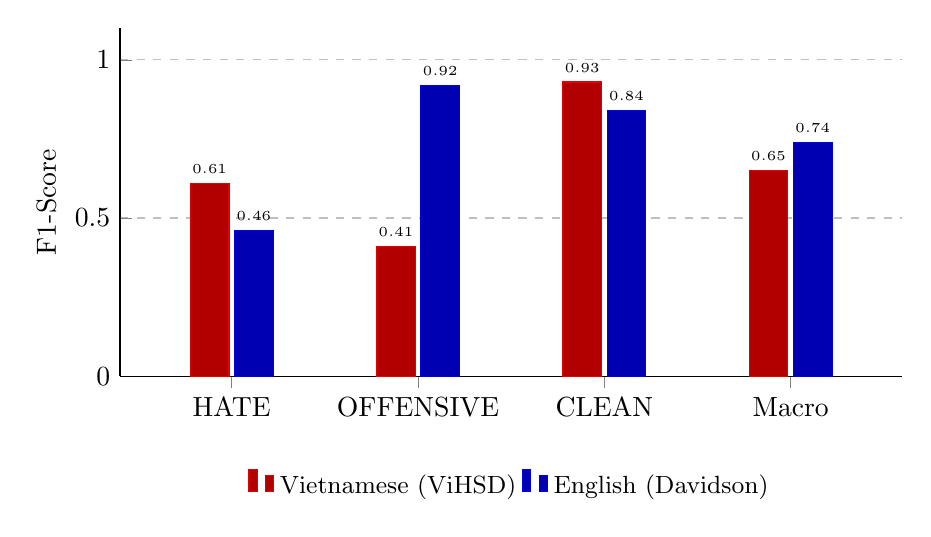
\begin{tikzpicture}
\begin{axis}[
    ybar,
    enlarge x limits=0.2,
    legend style={at={(0.5,-0.25)}, anchor=north, legend columns=-1, draw=none, font=\small},
    ylabel={F1-Score},
    symbolic x coords={HATE, OFFENSIVE, CLEAN, Macro},
    xtick=data,
    nodes near coords,
    nodes near coords align={vertical},
    every node near coord/.append style={font=\tiny\bfseries},
    ymin=0, ymax=1.1,
    width=0.95\textwidth,
    height=6cm,
    bar width=14pt,
    ymajorgrids=true,
    grid style=dashed,
    axis lines*=left,
]
\addplot[fill=red!70!black, draw=red!90!black] coordinates {(HATE,0.61) (OFFENSIVE,0.41) (CLEAN,0.93) (Macro,0.65)};
\addplot[fill=blue!70!black, draw=blue!90!black] coordinates {(HATE,0.46) (OFFENSIVE,0.92) (CLEAN,0.84) (Macro,0.74)};
\legend{Vietnamese (ViHSD), English (Davidson)}
\end{axis}
\end{tikzpicture}

    \caption{F1-score comparison per class and macro-average on the 1,000-sample mixed test set.}
    \label{fig:f1_comp}
\end{minipage}
\vspace{1em}
\begin{minipage}{0.95\textwidth}
    \centering
    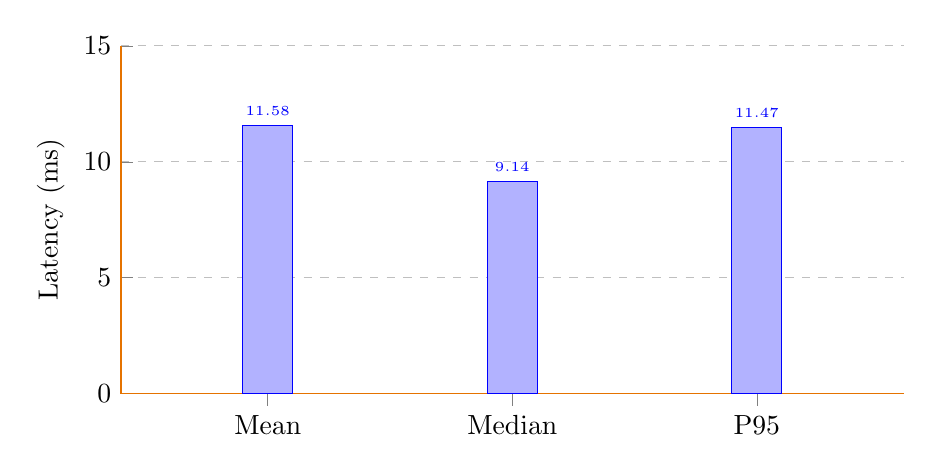
\begin{tikzpicture}
\begin{axis}[
    ybar,
    enlarge x limits=0.3,
    ylabel={Latency (ms)},
    symbolic x coords={Mean, Median, P95},
    xtick=data,
    nodes near coords,
    nodes near coords align={vertical},
    every node near coord/.append style={font=\tiny\bfseries},
    ymin=0, ymax=15,
    width=0.95\textwidth,
    height=6cm,
    bar width=18pt,
    fill=orange!80!black,
    draw=orange!90!black,
    ymajorgrids=true,
    grid style=dashed,
    axis lines*=left,
]
\addplot coordinates {(Mean,11.58) (Median,9.14) (P95,11.47)};
\end{axis}
\end{tikzpicture}

    \caption{End-to-end latency profile (ms) per request.}
    \label{fig:latency_fig}
\end{minipage}
\end{figure}
